\documentclass{article}
\usepackage{amsmath,amssymb,graphicx,enumitem,wrapfig}

\begin{document}
\parindent=0cm
\parskip=6pt
\pagestyle{empty}

%Begin
%Language English
%Source Cariboo College High School Mathematics competition
%Title Final Round 1973
%Question 1
%Subject geometry
%Category area
%Type MC
%Choices 5
%Answer B
%Creator Victor Semenoff
%Rdifficulty 29
%Qtext

\scriptsize
Source: Cariboo College High School Mathematics Contest

\normalsize
\begin{wrapfigure}[5]{r}[0pt]{0pt}
	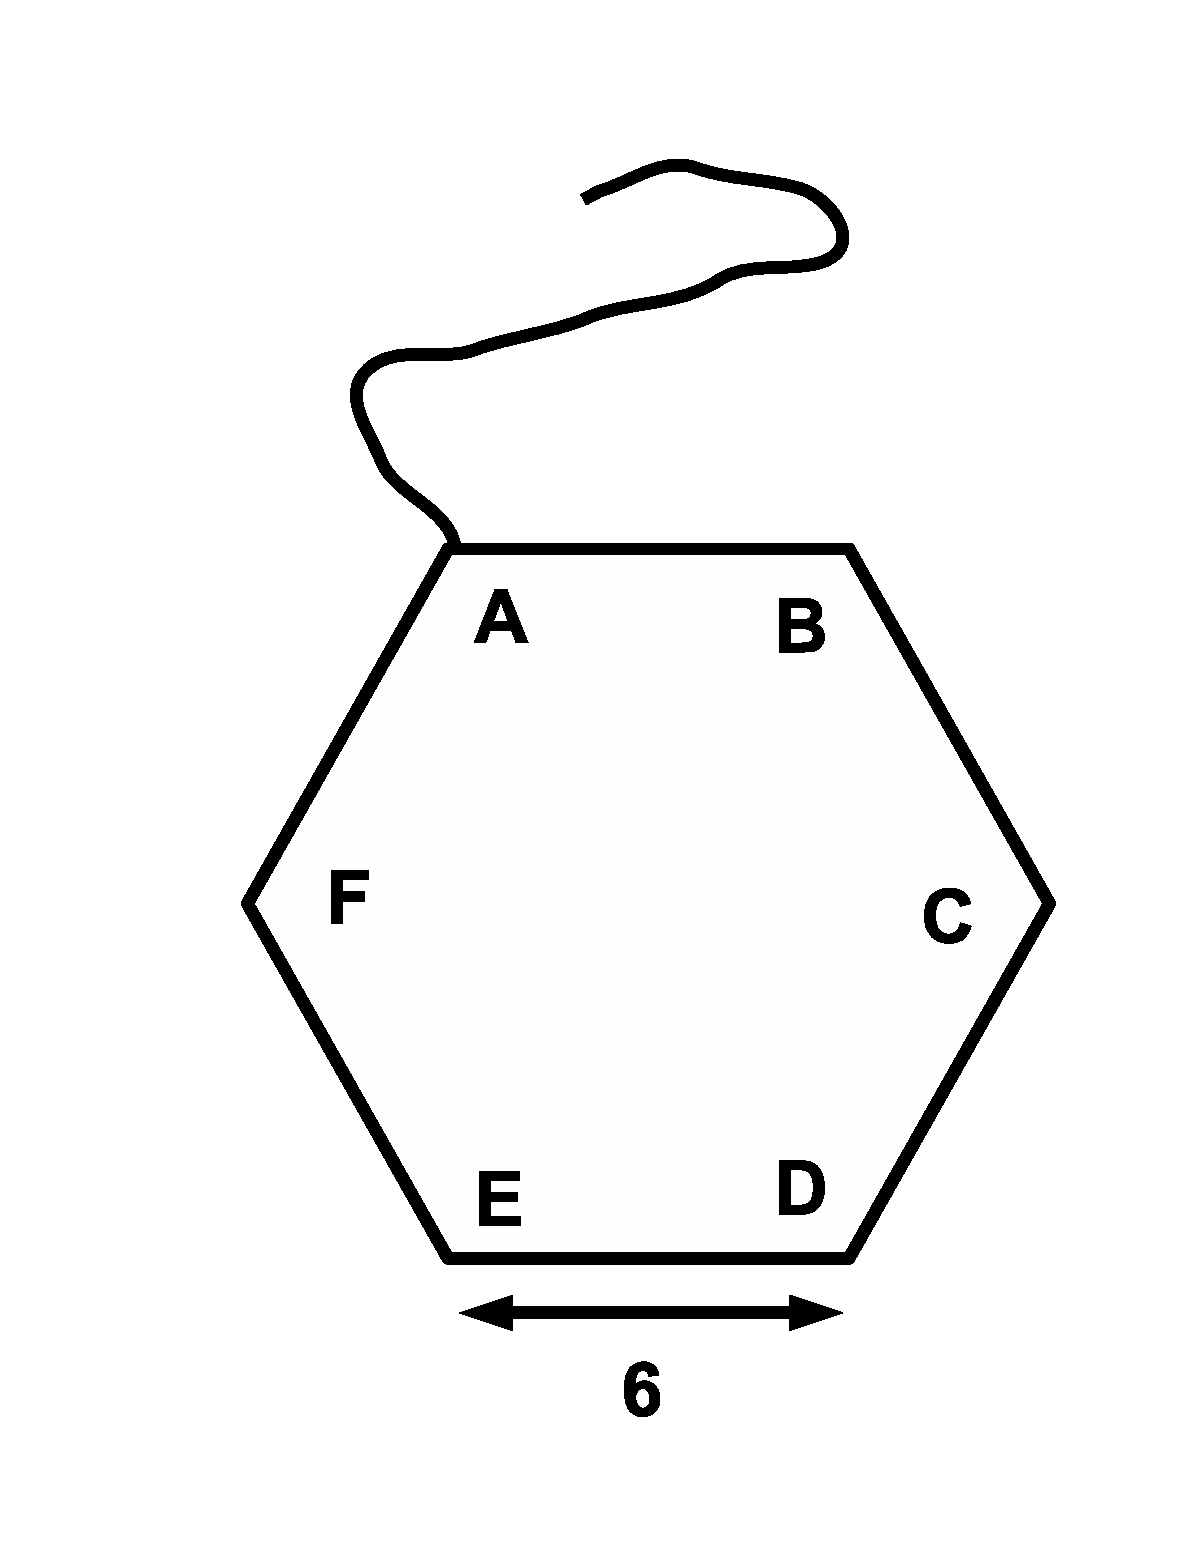
\includegraphics[width=20mm,viewport=89 57 506 671]{CCSFR73-1pic.eps}
\end{wrapfigure}
A steer is tethered to corner A of the the hexagonal silo in the figure.  If the length of each side of the regular hexagon is 6 and the length of the tether is one half the perimeter of the silo, find the area the steer can graze.\\
%ChoiceA
(A) 300$\pi$\\
%ChoiceB
(B) 276$\pi$\\
%ChoiceC
(C) 138$\pi$\\
%ChoiceD
(D) 12$\pi$\\
%ChoiceE
(E) Not enough information\\
%Ftext

\begin{wrapfigure}{r}[0pt]{0pt}
	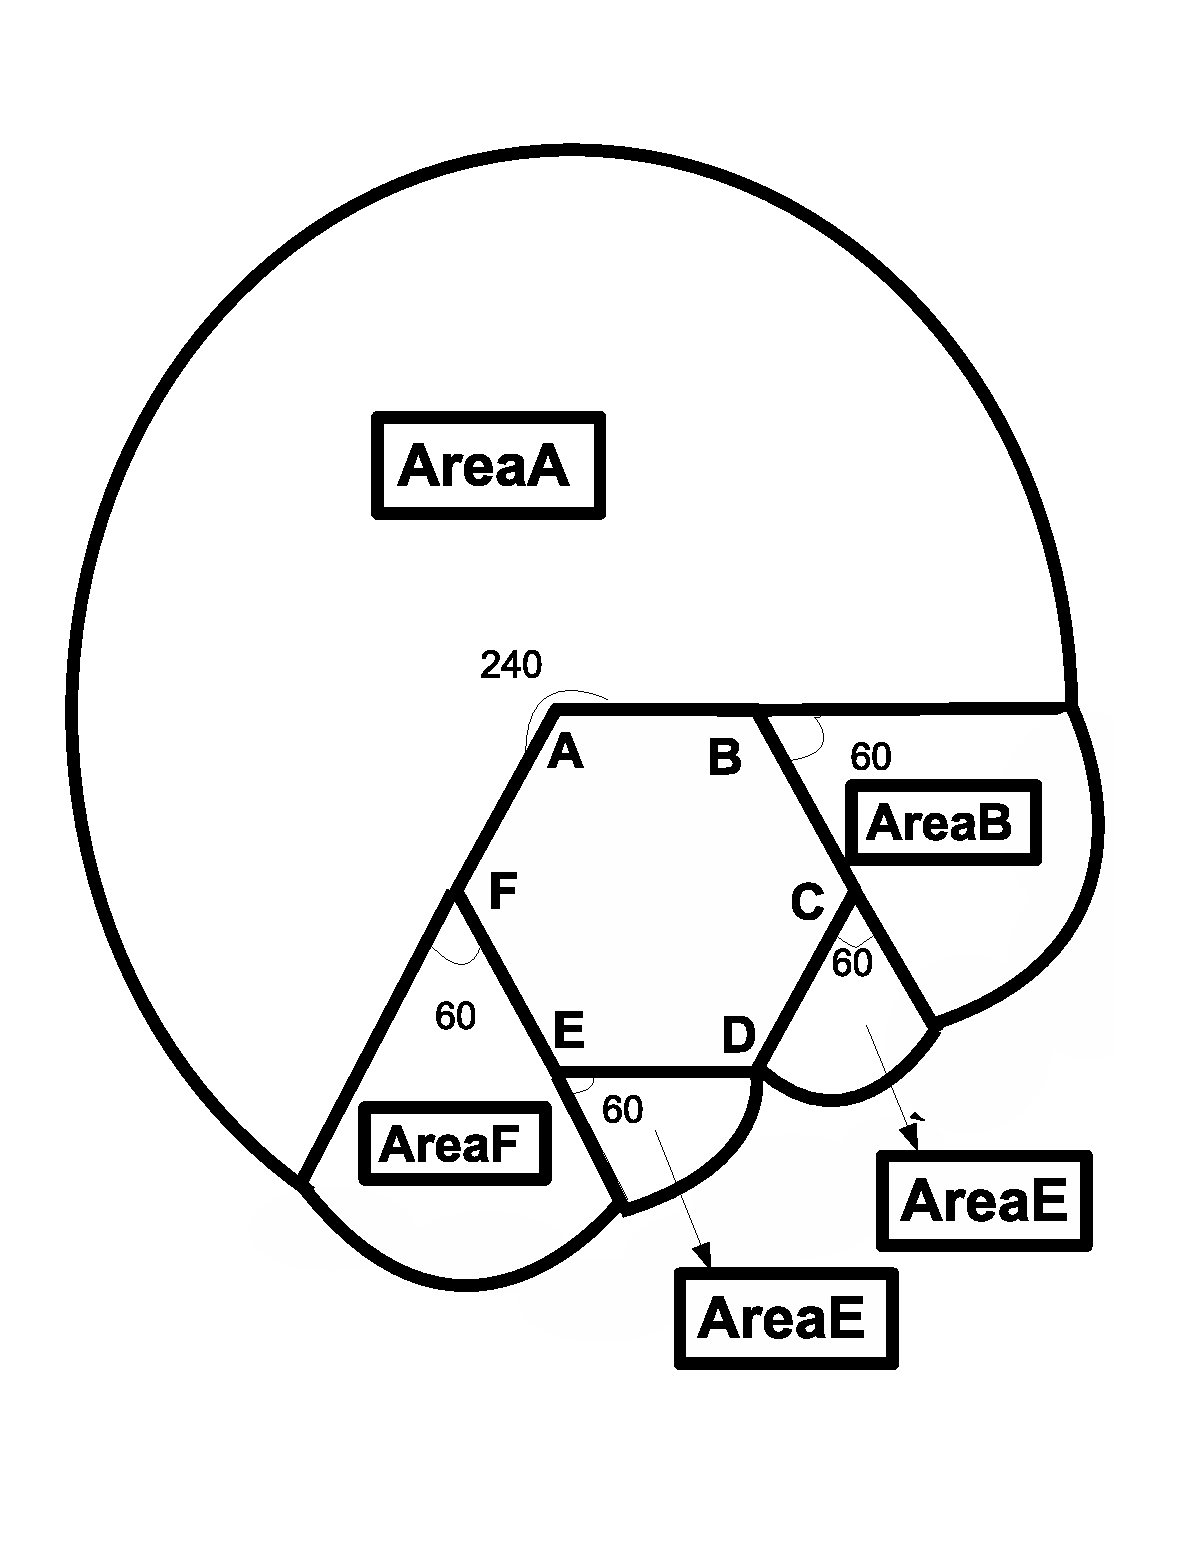
\includegraphics[width=30mm,viewport=18 78 525 628]{CCSFR73-1pic2.eps}
\end{wrapfigure}

\textbf{The correct answer is (B): 276$\pi$}\\[1 ex]
The hexagon is regular, so each side has length 6. The rope is $(6*6)/2=18$ long.  Each angle in a hexagon is $120\,^{\circ}$.  So there is a $240\,^{\circ}$ arc of length 18 centered at A.  Then there are also two $60\,^{\circ}$ arcs of length 12; one centered at B and one centered at F.  Finally, there are two $60\,^{\circ}$ arcs of length 6; one centered at C and one at E.\\[1 ex]
We sum the areas bounded by the arcs and the hexagon:
\begin{align*} 
\textrm{AreaA} &=(240\,^{\circ})/(360\,^{\circ})\times \pi(18)^2=216\pi\\
\textrm{AreaBF} &=2*(60\,^{\circ})/(360\,^{\circ})\times \pi(12)^2=48\pi\\
\textrm{AreaCE} &=2*(60\,^{\circ})/(360\,^{\circ})\times \pi(6)^2=12\pi\\
\end{align*}
Thus the total area is $=216\pi+48\pi+12\pi=276\pi$.
%End
\\[5 ex]
%Begin
%Language English
%Source Cariboo College High School Mathematics competition
%Title Final Round 1973
%Question 2 Part A
%Subject algebra
%Category modelling
%Type MC
%Choices 5
%Answer D
%Creator Victor Semenoff
%Rdifficulty 28
%Qtext

\scriptsize
Adapted From: Cariboo College High School Mathematics Contest

\normalsize
%\begin{wrapfigure}[2]{r}[0pt]{0pt}
%	\includegraphics[width=30mm,viewport=]{CCJ78-04}
%\end{wrapfigure}
A man has an orchard with three successive gates.  He posts a sign stating that a person may pick as many apples as he likes provided he returns $\frac{1}{2}$ an apple more than $\frac{1}{2}$ the apples in his possession at each gate as he exits.  It is not permitted to cut, eat, or deface the apples in any way; if these regulations are not observed, no apples can be taken.  If you wanted to leave with exactly one apple (exit through all 3 gates) , how many would you pick?\\
%ChoiceA
(A) 3 apples\\
%ChoiceB
(B) 7 apples\\
%ChoiceC
(C) 12 apples\\
%ChoiceD
(D) 15 apples\\
%ChoiceE
(E) 21 apples\\
%Ftext

%\begin{wrapfigure}{r}[0pt]{0pt}
%	\includegraphics[width=30mm,viewport=]{CCJ78-04}
%\end{wrapfigure}

\textbf{The correct answer is (D): 15 apples}\\[1 ex]
Let $a$ be the number of apples you enter a gate with, and let $x$ be the number of apples that you leave this gate with. According to the rules given, $x=a-(\frac{1}{2}a+\frac{1}{2})=\frac{1}{2}(a-1)$.
\\[2 ex]
Solving for $a$, we find that to leave a gate with $x$ apples you must enter it with $a$ apples such that $a=2x+1$.
\\[2 ex]
To leave the $3^{rd}$ gate with 1 apple, enter it with $2\times1+1=3$ apples.  This requires you to leave the second gate with 3 apples.  To do this, you must enter the $2^{nd}$ gate with $2\times3+1=7$ apples.  This requires you to leave the $1^{st}$ gate with 7 apples which, in turn, requires you to enter the $1^{st}$ gate with $2\times7+1=15$ apples.
%End
\\[5 ex]
%Begin
%Language English
%Source Cariboo College High School Mathematics competition
%Title Final Round 1973
%Question 2 Part B
%Subject algebra
%Category modelling
%Type MC
%Choices 5
%Answer D
%Creator Victor Semenoff
%Rdifficulty 30
%Qtext

\scriptsize
Adapted From: Cariboo College High School Mathematics Contest

\normalsize
%\begin{wrapfigure}[2]{r}[0pt]{0pt}
%	\includegraphics[width=30mm,viewport=]{CCJ78-04}
%\end{wrapfigure}
A man has an orchard with $n$ successive gates.  He posts a sign stating that a person may pick as many apples as he likes provided he returns $\frac{1}{2}$ an apple more than $\frac{1}{2}$ the apples in his possession at each gate as he exits.  It is not permitted to cut, eat, or deface the apples in any way; if these regulations are not observed, no apples can be taken.  If you wanted to leave with exactly one apple (exit through all $n$ gates) , how many apples would you pick?\\
%ChoiceA
(A) $n^{2}+1$ apples\\
%ChoiceB
(B) $n^{2}-1$ apples\\
%ChoiceC
(C) $2^{(n+1)}+1$ apples\\
%ChoiceD
(D) $2^{(n+1)}-1$ apples\\
%ChoiceE
(E) None of the above\\
%Ftext

%\begin{wrapfigure}{r}[0pt]{0pt}
%	\includegraphics[width=30mm,viewport=]{CCJ78-04}
%\end{wrapfigure}

\textbf{The correct answer is (D): $2^{(n+1)}-1$ apples}\\[1 ex]
Let $a$ be the number of apples you enter a gate with, and let $x$ be the number of apples that you leave this gate with. According to the rules given, $x=a-(\frac{1}{2}a+\frac{1}{2})=\frac{1}{2}(a-1)$. Solving for $a$, we find that to leave a gate with $x$ apples you must enter it with $a$ apples such that $a=2x+1$.\\
To leave the $n^{th}$ (last) gate with 1 apple, enter it with $2\times1+1=3$ apples.  This requires you to leave the second last ($(n-1)^{th}$) gate with 3 apples.  To do this, you must enter the $(n-1)^{th}$ gate with $2\times3+1=7$ apples.  This requires you to leave the $(n-2)^{nd}$ gate with 7 apples which, in turn, requires you to enter the $(n-2)^{nd}$ gate with $2\times7+1=15$ apples.\\
Continuing in this line, we find we need 3,7,15,31,63,127,... where the $m$-th term in the series tells you the number of apples you need to pick to pass through $m$ gates and leave with one apple.  Notice that the $m$-th term can be represented by $2^{(m+1)}-1$. Therefore, to pass through $n$ gates and leave with 1 apple enter the first gate with $2^{(n+1)}-1$ apples.
%End
\\[5 ex]
%Begin
%Language English
%Source Cariboo College High School Mathematics competition
%Title Final Round 1973
%Question 3 Part A
%Subject geometry
%Category length
%Type MC
%Choices 5
%Answer B
%Creator Victor Semenoff
%Rdifficulty 26
%Qtext

\scriptsize
Adapted From: Cariboo College High School Mathematics Contest

\normalsize
%\begin{wrapfigure}[2]{r}[0pt]{0pt}
%	\includegraphics[width=30mm,viewport=]{CCJ78-04}
%\end{wrapfigure}
A square of side length 24 is packed with four circles of equal diameter such that their centres lie on the diagonals of the square and each circle is tangent to two of the others. A circle centered at the centre of the square is drawn so that it is tangent to each of the four other circles. What is its radius?\\
%ChoiceA
(A) 6\\
%ChoiceB
(B) $6\sqrt{2}-6$\\
%ChoiceC
(C) $6+\sqrt{2}$\\
%ChoiceD
(D) $6+2\sqrt{2}$\\
%ChoiceE
(E) Not enough information\\
%Ftext

%\begin{wrapfigure}{r}[0pt]{0pt}
%	\includegraphics[width=30mm,viewport=]{CCJ78-04}
%\end{wrapfigure}

\textbf{The correct answer is (B): $6\sqrt{2}-6$}\\[1 ex]
Let $r$ be the radius of the smaller circle and let $R$ be the radius common to the four large circles. Choose a large circle and call it $A$. Draw a line segment connecting the centre of the small circle with the centre of $A$. Now let $X$ be a point where $A$ is tangent to another large circle. Draw a radius of $A$ to $X$ and a segment from the centre of the small circle to $X$. It forms an isosceles right triangle. Thus, from the triangle, $R^{2}+R^{2}=(R+r)^2$ or $R+r=R\sqrt{2}$.  Solving for R gives
\begin{equation*}
r=(\sqrt{2}-1)R.
\end{equation*}
Now, $R$ is one quarter the length of the square, so $R=6$ and 
\begin{equation*}
r=(\sqrt{2}-1)6=6\sqrt{2}-6.
\end{equation*}
%End
\\[5 ex]
%Begin
%Language English
%Source Cariboo College High School Mathematics competition
%Title Final Round 1973
%Question 3 Part B
%Subject geometry
%Category length
%Type MC
%Choices 5
%Answer B
%Creator Victor Semenoff
%Rdifficulty 29
%Qtext

\scriptsize
Adapted From: Cariboo College High School Mathematics Contest

\normalsize
%\begin{wrapfigure}[2]{r}[0pt]{0pt}
%	\includegraphics[width=30mm,viewport=]{CCJ78-04}
%\end{wrapfigure}
A square of side length $x$ is packed with four circles of equal diameter such that their centres lie on the diagonals of the square and each circle is tangent to two of the others. A circle centered at the centre of the square is drawn so that it is tangent to each of the four other circles. What is its radius?\\
%ChoiceA
(A) $\frac{x}{4}$\\
%ChoiceB
(B) $\frac{x}{4}\sqrt{2}-\frac{x}{4}$\\
%ChoiceC
(C) $x+\sqrt{2}$\\
%ChoiceD
(D) $x+2\sqrt{2}$\\
%ChoiceE
(E) Not enough information\\
%Ftext

%\begin{wrapfigure}{r}[0pt]{0pt}
%	\includegraphics[width=30mm,viewport=]{CCJ78-04}
%\end{wrapfigure}

\textbf{The correct answer is (B): $\frac{x}{4}\sqrt{2}-\frac{x}{4}$}\\[1 ex]
Let $r$ be the radius of the smaller circle, and $R$ be the radius common to the four large circles. Choose a large circle and call it $A$. Draw a line segment connecting the centre of the small circle with the centre of $A$. Now let $X$ be a point where $A$ is tangent to another large circle. Draw a radius of $A$ to $X$ and a segment from the centre of the small circle to $X$. It forms an isosceles right triangle. Thus, from the triangle, $R^{2}+R^{2}=(R+r)^2$ or $R+r=R\sqrt{2}$.  Solving for r gives
\begin{equation*}
r=(\sqrt{2}-1)R.
\end{equation*}
Now, $R$ is one quarter the length of the square, so $R=\frac{x}{4}$ and 
\begin{equation*}
r=(\sqrt{2}-1)\frac{x}{4}=\frac{x}{4}\sqrt{2}-\frac{x}{4}.
\end{equation*}
%End
\\[5 ex]
%Begin
%Language English
%Source Cariboo College High School Mathematics competition
%Title Final Round 1973
%Question 4
%Subject algebra
%Category modelling
%Type MC
%Choices 5
%Answer A
%Creator Victor Semenoff
%Rdifficulty 29
%Qtext

\scriptsize
Adapted From: Cariboo College High School Mathematics Contest

\normalsize
%\begin{wrapfigure}[2]{r}[0pt]{0pt}
%	\includegraphics[width=30mm,viewport=]{CCJ78-04}
%\end{wrapfigure}
A railway worker is $\frac{3}{8}$ of the way across a bridge when he hears a train coming behind him.  If the train is traveling at 60 mi/h and the man can run to either end of the bridge just in time to save his life, how fast (in mi/h) can he run?\\
%ChoiceA
(A) 15\\
%ChoiceB
(B) 20\\
%ChoiceC
(C) 30\\
%ChoiceD
(D) 10\\
%ChoiceE
(E) 5\\
%Ftext

%\begin{wrapfigure}{r}[0pt]{0pt}
%	\includegraphics[width=30mm,viewport=]{CCJ78-04}
%\end{wrapfigure}

\textbf{The correct answer is (A): 15}\\[1 ex]
Let $l$ be the length of the bridge. The railway worker is $\frac{3}{8}l$ from the end where the train is approaching, and $\frac{5}{8}l$ from the other end of the bridge. Thus, in the time it takes the man to run to the near end, the train would have arrived at the bridge. If the man had run to the far end , he would still have $\frac{5}{8}l-\frac{3}{8}l=\frac{1}{4}l$ to travel when the train reached the bridge. 

The worker and the train reach the far end at the same time, thus the worker travels $\frac{1}{4}l$ in the same amount of time that the train travels $l$. So the worker is $\frac{1}{4}$ as fast as the train, or 15 mi/h.
%End
\\[5 ex]
%Begin
%Language English
%Source Cariboo College High School Mathematics competition
%Title Final Round 1973
%Question 5 Part A
%Subject algebra
%Category modelling
%Type MC
%Choices 5
%Answer D
%Creator Victor Semenoff
%Rdifficulty 28
%Qtext

\scriptsize
Adapted From: Cariboo College High School Mathematics Contest

\normalsize
%\begin{wrapfigure}[2]{r}[0pt]{0pt}
%	\includegraphics[width=30mm,viewport=]{CCJ78-04}
%\end{wrapfigure}
This problem comes from the Greeks:

`I am a brazen lion, a fountain; my spouts are my two eyes, my mouth, and the flat of my right foot. My right eye fills a jar in one day, my left eye in one and a half days, and my foot in two days; my mouth is capable of filling it in three hours. Tell me how long it will take to fill it.'\\
%ChoiceA
(A) 1 day\\
%ChoiceB
(B) $\frac{1}{8}$ day\\
%ChoiceC
(C) $\frac{11}{70}$ day\\
%ChoiceD
(D) $\frac{6}{61}$ day\\
%ChoiceE
(E) None of these.\\
%Ftext

%\begin{wrapfigure}{r}[0pt]{0pt}
%	\includegraphics[width=30mm,viewport=]{CCJ78-04}
%\end{wrapfigure}

\textbf{The correct answer is (D): $\frac{6}{61}$ day}\\[1 ex]
Let $r_{r}$, $r_{l}$, $r_{f}$, and $r_{m}$ be the rate at which the lion's right eye, left eye, right foot, and mouth fill the jar, respectively. Since the left eye could fill the jar in $\frac{3}{2}$ the time the right eye could, its rate is $r_{l}=\frac{2}{3}r_{r}$. Similarly, in terms of the right eye, we have the foot $r_{f}=\frac{1}{2}r_{r}$, and the mouth $r_{m}=8r_{r}$.  When we put all four together we get the combined rate
\begin{equation*}
r_{r}+r_{l}+r_{f}+r_{m}=r_{r}+\frac{2}{3}r_{r}+\frac{1}{2}r_{r}+8r_{r}=\frac{61}{6}r_r.
\end{equation*}
Since the rate the right eye fills the jar is 1 jar per day, we have the total rate of $\frac{61}{6}$ jars per day, and thus it takes $\frac{6}{61}$ day to fill the jar.
%End
\\[5 ex]
%Begin
%Language English
%Source Cariboo College High School Mathematics competition
%Title Final Round 1973
%Question 5 Part B
%Subject algebra
%Category modelling
%Type MC
%Choices 5
%Answer D
%Creator Victor Semenoff
%Rdifficulty 26
%Qtext

\scriptsize
Adapted From: Cariboo College High School Mathematics Contest

\normalsize
%\begin{wrapfigure}[2]{r}[0pt]{0pt}
%	\includegraphics[width=30mm,viewport=]{CCJ78-04}
%\end{wrapfigure}
Four spouts separately fill a jar.  The first on takes 1 day to fill the jar, the second one one and a half days, the third one 12 hours and the fourth one 3 hours.  If all four spouts are used at the same time, how long will it take to fill the jar?\\
%ChoiceA
(A) 1 day\\
%ChoiceB
(B) $\frac{1}{8}$ day\\
%ChoiceC
(C) $\frac{11}{70}$ day\\
%ChoiceD
(D) $\frac{3}{35}$ day\\
%ChoiceE
(E) None of these.\\
%Ftext

%\begin{wrapfigure}{r}[0pt]{0pt}
%	\includegraphics[width=30mm,viewport=]{CCJ78-04}
%\end{wrapfigure}

\textbf{The correct answer is (D): $\frac{3}{35}$ day}\\[1 ex]
Let $r_{1}$, $r_{2}$, $r_{3}$, and $r_{4}$ be the rate at which the first, second, third and fourth spouts fill the jar, respectively. Since the second spout could fill the jar in $\frac{3}{2}$ the time the first could, its rate is $r_{2}=\frac{2}{3}r_{1}$. Similarly, in terms of the first spout, we have the third $r_{3}=2r_{1}$, and the fourth $r_{4}=8r_{1}$.  When we put all four together we get the combined rate
\begin{equation*}
r_{1}+r_{2}+r_{3}+r_{4}=r_{1}+\frac{2}{3}r_{1}+2r_{1}+8r_{1}=\frac{35}{3}r_1.
\end{equation*}
Since the rate the first spout fills the jar is 1 jar per day, we have the total rate of $\frac{35}{3}$ jars per day, and thus it takes $\frac{3}{35}$ of a day to fill a jar.
%End
\\[5 ex]
%Begin
%Language English
%Source Cariboo College High School Mathematics competition
%Title Final Round 1973
%Question 6
%Subject logic
%Category general
%Type MC
%Choices 5
%Answer B
%Creator Victor Semenoff
%Rdifficulty 25
%Qtext

\scriptsize
Adapted From: Cariboo College High School Mathematics Contest

\normalsize
%\begin{wrapfigure}[2]{r}[0pt]{0pt}
%	\includegraphics[width=30mm,viewport=]{CCJ78-04}
%\end{wrapfigure}
Three men, Able, Baker, and Charlie, make comments about each other. Able says, ``Baker is a liar''; Baker says, ``Charlie is a liar''; and Charlie says, ``Both Able and Baker are liars.'' Who is telling the truth?\\
%ChoiceA
(A) Able\\
%ChoiceB
(B) Baker\\
%ChoiceC
(C) Charlie\\
%ChoiceD
(D) Able and Baker\\
%ChoiceE
(E) None of them.\\
%Ftext

%\begin{wrapfigure}{r}[0pt]{0pt}
%	\includegraphics[width=30mm,viewport=]{CCJ78-04}
%\end{wrapfigure}

\textbf{The correct answer is (B): Baker}\\[1 ex]
Start by assuming Able is telling the truth. This means that Baker is lying, and thus Charlie is telling the truth. But Charlie says Able is lying, which contradicts the assumption that Able is telling the truth.

Thus we know that Able is lying. And thus Baker is telling the truth, and because of this Charlie is lying.
%End
\\[5 ex]
%Begin
%Language English
%Source Cariboo College High School Mathematics competition
%Title Final Round 1973
%Question 8
%Subject algebra
%Category modelling
%Type MC
%Choices 5
%Answer E
%Creator Victor Semenoff
%Rdifficulty 30
%Qtext

\scriptsize
Adapted From: Cariboo College High School Mathematics Contest

\normalsize
%\begin{wrapfigure}[2]{r}[0pt]{0pt}
%	\includegraphics[width=30mm,viewport=]{CCJ78-04}
%\end{wrapfigure}
A boy in a department store, noticing the down escalator in motion, raises the question ``How many steps are there in the escalator between the floors?'' He walked all the way down the escalator as it was in motion and found that when he walked 20 steps it took him 35 seconds. Upon doing it a second time he found that when he took 28 steps it took him 30 seconds to get all the way down. What is the answer to the boy's question?\\
%ChoiceA
(A) 64\\
%ChoiceB
(B) 45\\
%ChoiceC
(C) 36\\
%ChoiceD
(D) 95\\
%ChoiceE
(E) 76\\
%Ftext

%\begin{wrapfigure}{r}[0pt]{0pt}
%	\includegraphics[width=30mm,viewport=]{CCJ78-04}
%\end{wrapfigure}

\textbf{The correct answer is (E): 76}\\[1 ex]
Let $s$ be the number of steps on the escalator, and let $r$ be the number of steps the escalator moves down per second. When the boy walks 20 steps he will have moved down a total of $20+35r$ steps. Since this takes him to the bottom, we have $s=20+35r$.  Solving for $r$ gives
\begin{equation*}
r=\frac{s-20}{35}
\end{equation*}
Similarly when the boy walks 28 steps he will have moved down a total of $s=28+30r$. Solving for $r$ gives
\begin{equation*}
r=\frac{s-28}{30}
\end{equation*}
Setting the two solutions for $r$ equal we find:
\begin{align*}
\frac{s-20}{35}&=r=\frac{s-28}{30}\\
30s-600&=35s-980\\
5s&=380\\
s&=76
\end{align*}
Thus there are 76 steps on the escalator.
%End
\\[5 ex]
%Begin
%Language English
%Source Cariboo College High School Mathematics competition
%Title Final Round 1973
%Question 10 Part A
%Subject geometry
%Category 3D
%Type MC
%Choices 5
%Answer C
%Creator Victor Semenoff
%Rdifficulty 33
%Qtext

\scriptsize
Adapted From: Cariboo College High School Mathematics Contest

\normalsize
\begin{wrapfigure}[5]{r}[0pt]{0pt}
	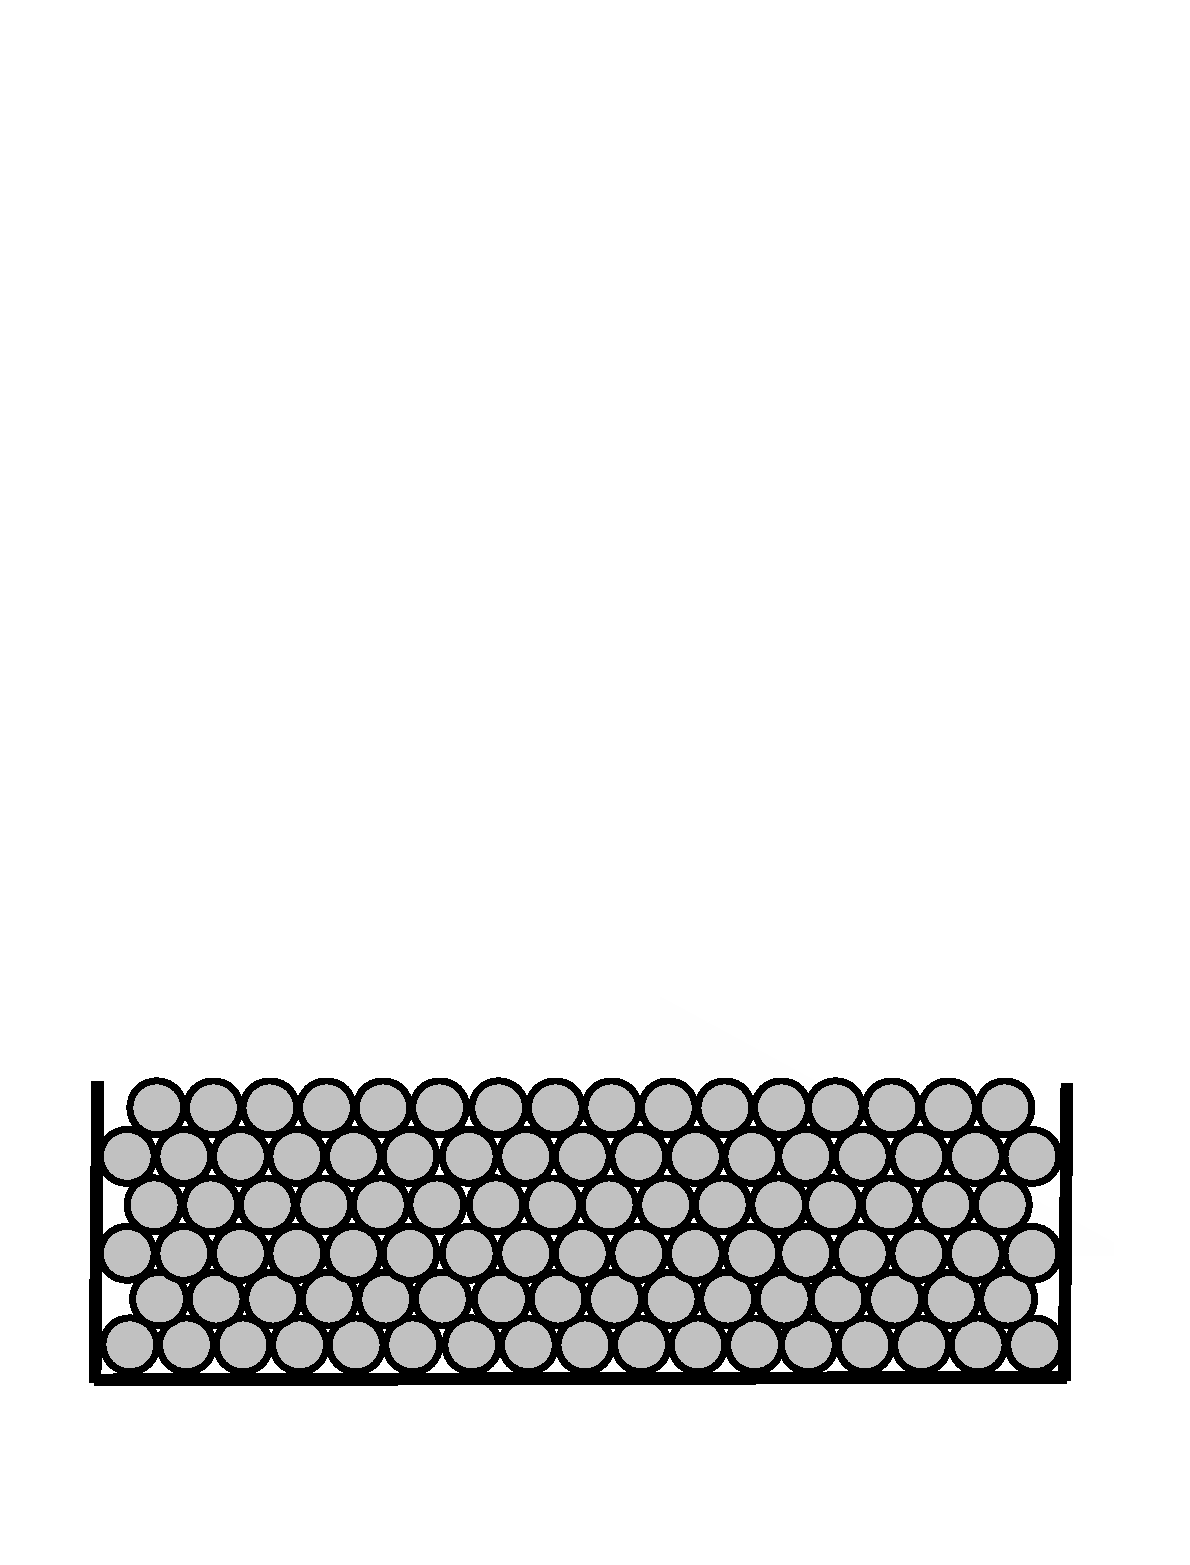
\includegraphics[width=30mm,viewport=27 69 511 230]{CCFR73-10pic1.eps}
\end{wrapfigure}
A \textbf{cube} shaped box of side length 24 is filled with spherical ball bearings of diameter 2. The bearings are arranged in horizontal layers, one on top of the other so that each ball is in contact with four in the next lower layer, four in the same layer, and four in the next higher layer (except of course, those in the bottom and top layers or adjacent to the sides of the box). This type of packing is known as normal piling or spherical close-packing. Find the number of ball bearings with which the box may be filled so that a lid may be placed on the box.\\
%ChoiceA
(A) 1728\\
%ChoiceB
(B) 2304\\
%ChoiceC
(C) 2120\\
%ChoiceD
(D) 1584\\
%ChoiceE
(E) None of these\\
%Ftext

\begin{wrapfigure}[8]{r}[0pt]{0pt}
	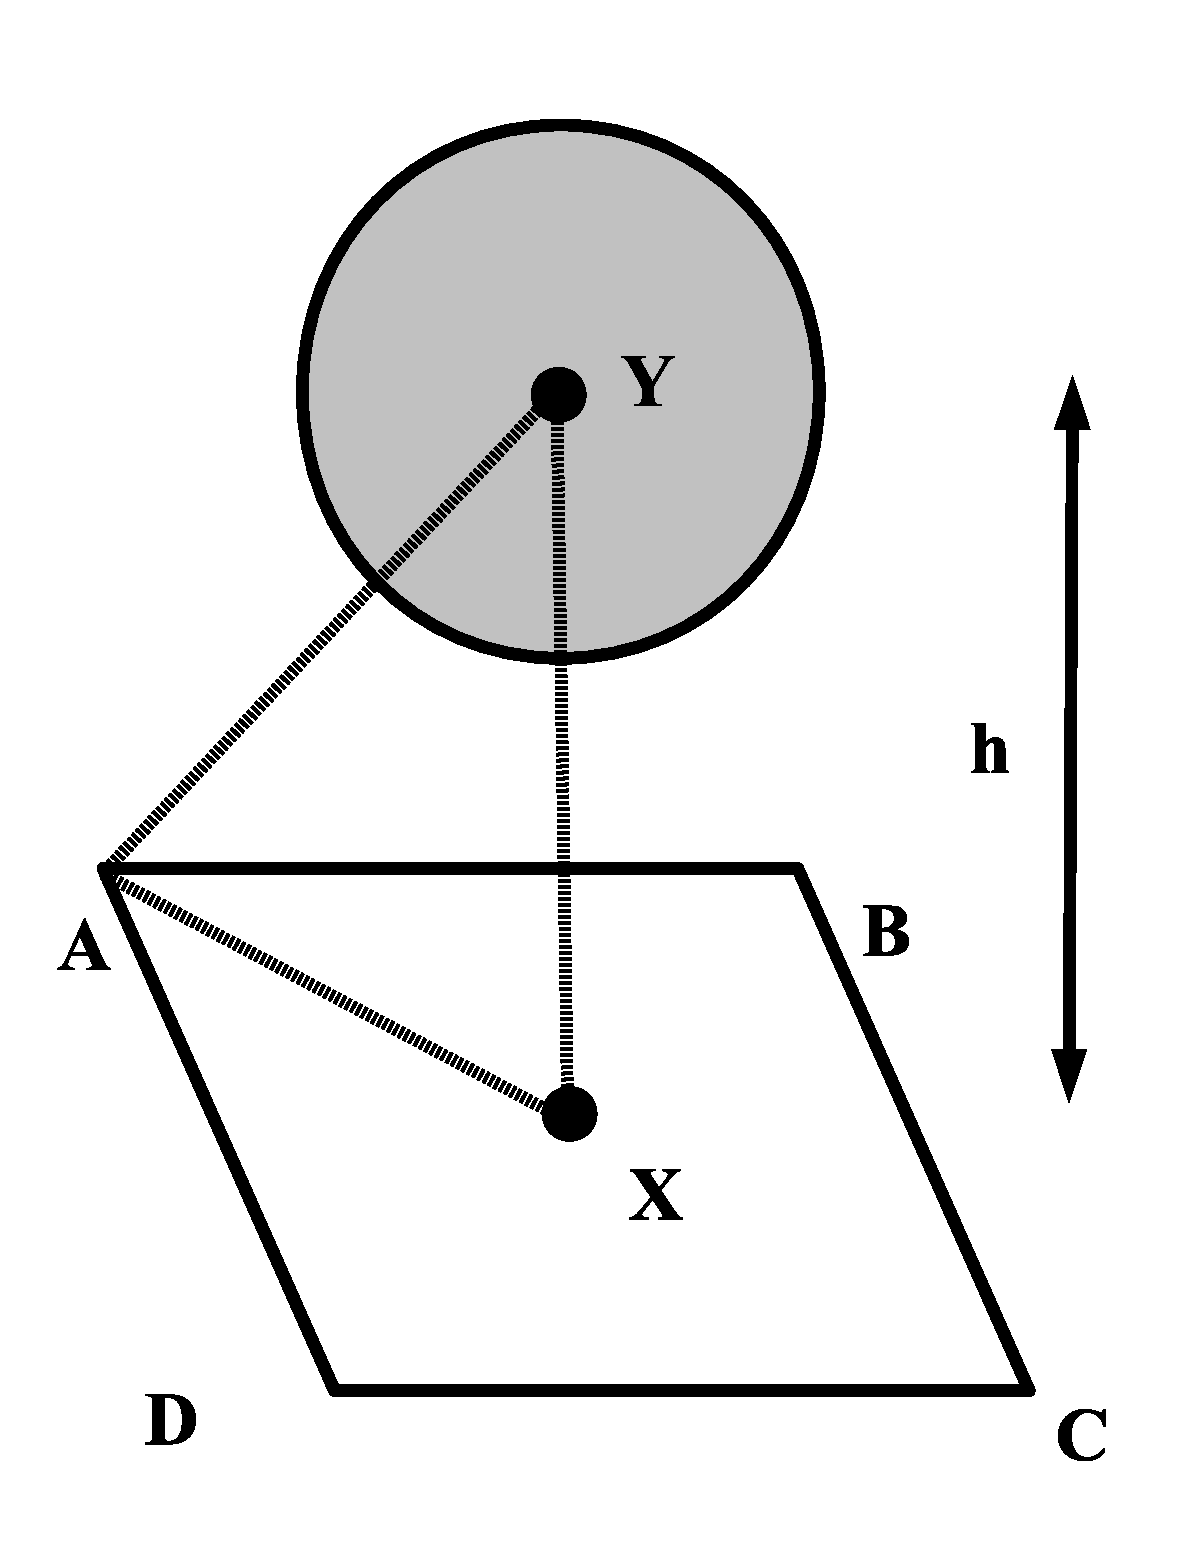
\includegraphics[width=24mm,viewport=14 42 526 688]{CCFR73-10pic3.eps}
\end{wrapfigure}

\textbf{The correct answer is (C): 2120}\\[1 ex]
Let $n$ be the number of layers of spheres that can fit into the box, h be the distance between layers (measured from planes passing through the centers of spheres in each layer), ABCD be a square formed by connecting the centers of four adjacent spheres in a layer, X be the center of the square, and let Y be the center of the sphere in the layer above that touches all four spheres. AX is half the length of the diagonal of the square, or $\frac{2\sqrt{2}}{2}=\sqrt{2}$. The length of AY is two radii, or 2. XY is of course h. AXY is a right triangle with hypotenuse AY=2, thus we have $\textrm{h}^{2}+2=4$, or h=$\sqrt{2}$.

Now, the total height occupied by the spheres is $2+(n-1)\textrm{h}$ (a quick sketch will convince you this is so). And we require the total height be less than 24, thus
\begin{equation*} 
2+(n-1)\textrm{h} \leq 24 \quad\textrm{gives}\quad n \leq1+11\sqrt{2}=16.5.
\end{equation*}
Thus 16 layers of spheres can be placed in the box. Finally, odd layers will have $12\times12=144$ spheres and even layers will have $11\times11=121$ spheres, thus there are $8\times144+8\times121=2120$ spheres that can fit in the box using normal piling.
%End
\\[5 ex]
%Begin
%Language English
%Source Cariboo College High School Mathematics competition
%Title Final Round 1973
%Question 10 Part B
%Subject geometry
%Category 3D
%Type MC
%Choices 5
%Answer C
%Creator Victor Semenoff
%Rdifficulty 31
%Qtext

\scriptsize
Adapted From: Cariboo College High School Mathematics Contest

\normalsize
\begin{wrapfigure}[5]{r}[0pt]{0pt}
	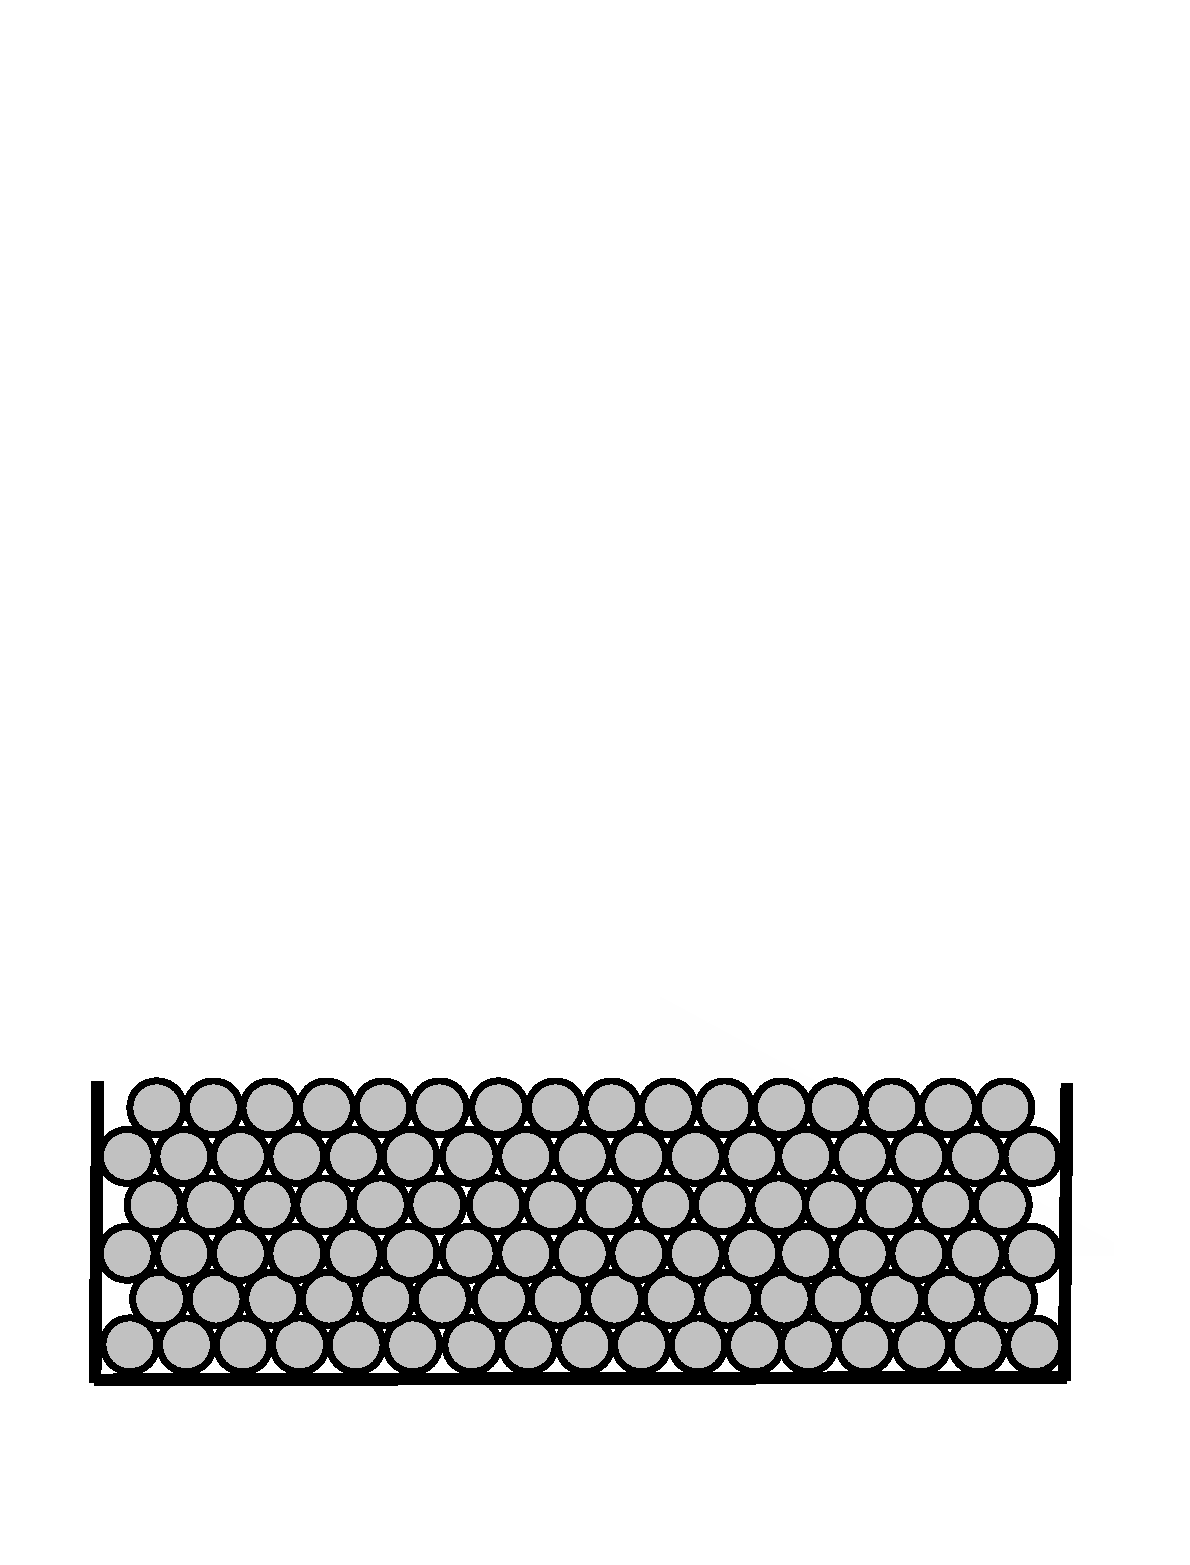
\includegraphics[width=30mm,viewport=27 69 511 230]{CCFR73-10pic1.eps}
\end{wrapfigure}
A \textbf{cube} shaped box of side length 24 is filled with spherical ball bearings of diameter 2. The bearings are arranged in horizontal layers, one on top of the other so that each ball is in contact with four in the next lower layer, four in the same layer, and four in the next higher layer (except of course, those in the bottom and top layers or adjacent to the sides of the box). This type of packing is known as normal piling or spherical close-packing. Find the number of layers of ball bearings with which the box may be filled so that a lid may be placed on the box.\\
%ChoiceA
(A) 12\\
%ChoiceB
(B) 15\\
%ChoiceC
(C) 16\\
%ChoiceD
(D) 18\\
%ChoiceE
(E) 24\\
%Ftext

\begin{wrapfigure}[8]{r}[0pt]{0pt}
	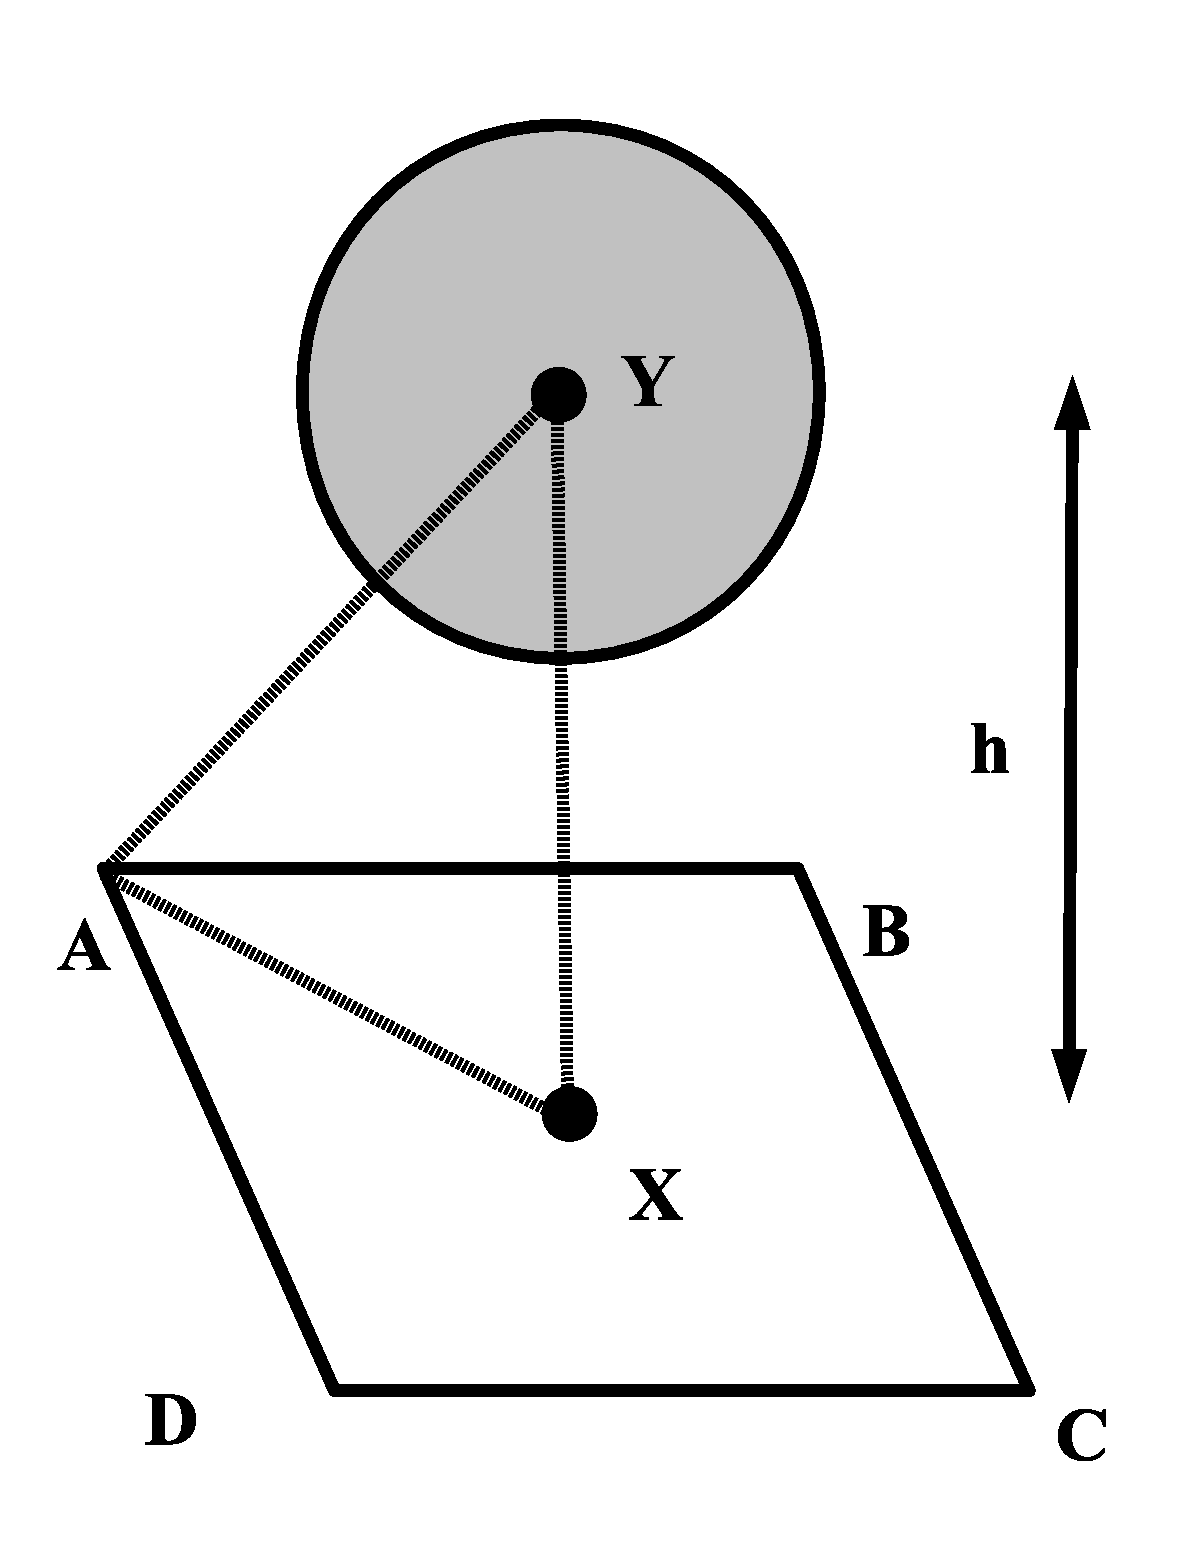
\includegraphics[width=24mm,viewport=14 42 526 688]{CCFR73-10pic3.eps}
\end{wrapfigure}

\textbf{The correct answer is (C): 16}\\[1 ex]
Let $n$ be the number of layers of spheres that can fit into the box, h the distance between layers (measured from planes passing through the centers of spheres in each layer), ABCD a square formed by connecting the centers of four adjacent spheres in a layer, X be the center of the square, and let Y be the center of the sphere in the layer above that touches all four spheres. AX is half the length of the diagonal of the square, or $\frac{2\sqrt{2}}{2}=\sqrt{2}$. The length of AY is two radii, or 2. XY is of course h. AXY is a right triangle with hypotenuse AY=2, thus we have $\textrm{h}^{2}+2=4$, or h=$\sqrt{2}$.

Now, the total height occupied by the spheres is $2+(n-1)\textrm{h}$ (a quick sketch will convince you this is so). And we require the total height be less than 24, thus
\begin{equation*} 
2+(n-1)\textrm{h} \leq 24 \quad\textrm{gives}\quad n \leq1+11\sqrt{2}=16.5.
\end{equation*}
Therefore 16 layers of spheres can be placed in the box. 
%End
\end{document}
